\documentclass{article}
% Choose a conveniently small page size
% PACKAGES
\usepackage[margin = 1in]{geometry}
\usepackage{amsfonts}
\usepackage{amsmath}
\usepackage{amssymb}
\usepackage{multicol}
\usepackage{graphicx}
\usepackage{float}
\usepackage{xcolor}
\usepackage{amsthm}
\usepackage{dsfont}
\usepackage{hyperref}

% MACROS
% Set Theory
\def\N{\mathbb{N}}
\def\R{\mathbb{R}}
\def\C{\mathbb{C}}
\def\Z{\mathbb{Z}}
%\def\^{\hat}
\def\-{\vec}
\def\d{\partial}
\def\!{\boldsymbol}
\def\X{\times}
%\def\-{\bar}
\def\bf{\textbf}
\def\l{\left}
\def\r{\right}
\title{Summer Internship for Damien Beecroft}
\author{Advisors: Amanda Howard, Panos Stinis}
\begin{document}
\maketitle
Physics-informed neural networks, or PINNs, have shown great promise in learning the solution to partial differential equations. However, there are still cases where PINNs fail to train. This summer, we will develop new techniques for cases where PINNs fail to train.
\par This document serves only as a suggested outline, and creativity is encouraged. The remaining weeks will be filled in as we see how the results develop. Many extensions are possible, including training deep operator networks (DeepONets) for a range of input parameters, or switching to model other dynamical systems. 
\par The suggested reading for each week consists of background information that you may find helpful as you work. I suggest you write a short, 1-2 sentence, summary of each paper and add it a working document after reading each paper. This will be the introduction to your final report, and later the introduction for a publication based on your work. Articles are available through PNNL when you’re logged into the VPN.
\begin{figure}[H]
\center
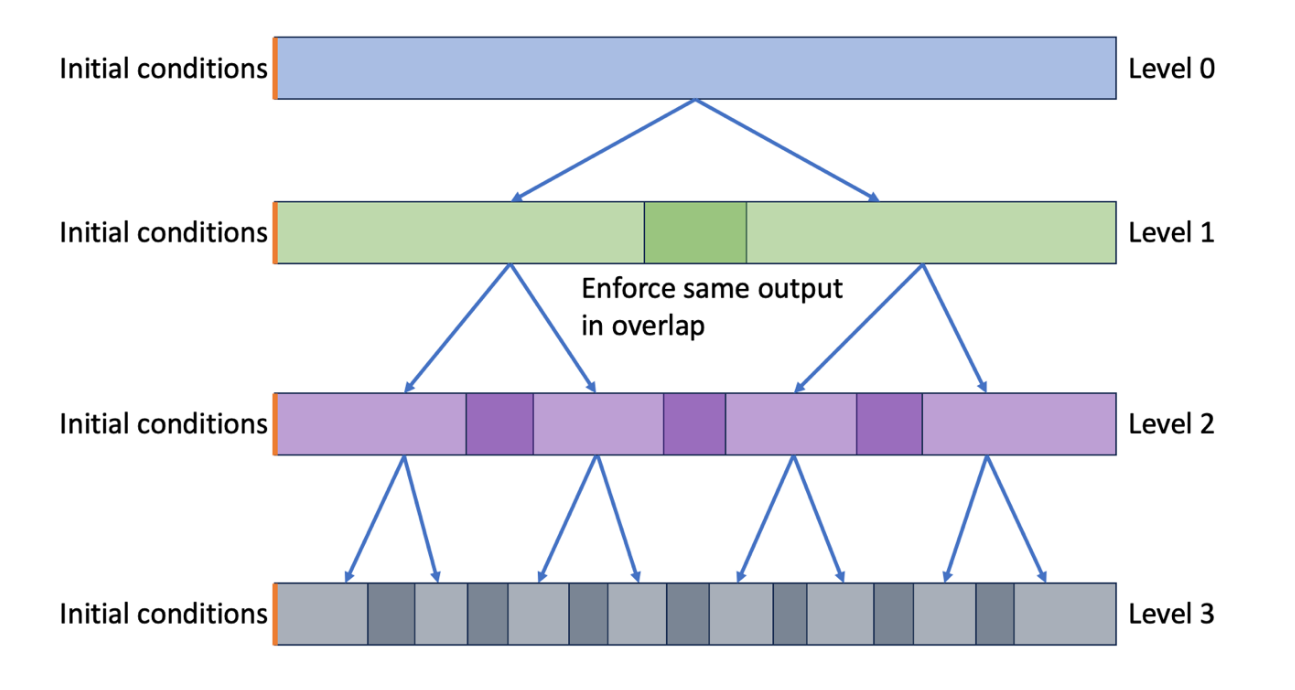
\includegraphics[width=0.8\textwidth]{imgs/domain_decomp}
\end{figure}
We will consider a multifidelity domain decomposition approach, where a PINN is trained in the full domain first. Then, the full domain training is used as a low fidelity prediction for a prediction in a subdivided domain. Two PINNs are trained in level 1, and the domains overlap so initial conditions are not needed to train the subdomain that occurs for later time. This process is repeated until the desired accuracy is reached across the domain.  
\par We will be working with Alexander Heinlein, who is an expert in domain decomposition. We will start by testing this setup on the case of an undamped pendulum, to see if we can overcome the issue of converging to fixed points for long time. If successful, we will move to more complex examples. Creativity is encouraged in designing training algorithms. 
\newpage
\subsection*{To Do}
\bf{Reading}:
\begin{itemize}
	\item How and Why PINNs Fail to Train: \url{https://arxiv.org/pdf/2007.14527.pdf}
	\begin{itemize}
		\item Neural Tangent Kernel Convergence and Generalization: \url{https://arxiv.org/abs/1806.07572}
		\item Deep Neural Networks as Gaussian Processes: \url{https://arxiv.org/abs/1711.00165}
	\end{itemize}
	\item A Method for Representing Periodic Functions and Enforcing
Exactly Periodic Boundary Conditions with Deep Neural Networks: \url{https://arxiv.org/pdf/2007.07442.pdf}
	\item Parallel Physics-Informed Neural Networks via Domain Decomposition: \url{https://arxiv.org/pdf/2104.10013.pdf}
	\item Fourier Analysis Sheds Light on Deep Neural Networks: \url{https://arxiv.org/abs/1901.06523}
\end{itemize}
\bf{Computing}:
\begin{itemize}

\item Run Amanda's code on Marianas
\end{itemize}

\newpage
\subsection*{Week 1}
\bf{Videos}:
\begin{itemize}
	\item Stanford CS229M Lecture 13 (Neural Tangent Kernel): \url{https://www.youtube.com/watch?v=btphvvnad0A&list=RDCMUCBa5G_ESCn8Yd4vw5U-gIcg&index=1}
\end{itemize}
\bf{Reading}:
\begin{itemize}
	\item PINNs: \url{https://www.sciencedirect.com/science/article/pii/S0021999118307125}
	\item Multifidelity PINN: \url{https://arxiv.org/pdf/1903.00104.pdf}
	\item Multifidelity DeepONets: \url{https://arxiv.org/pdf/2204.09157.pdf}
	\item Multifidelity Continual Learning: \url{https://arxiv.org/pdf/2304.03894.pdf}
	\item Fixed points and PINNs: \url{https://arxiv.org/pdf/2203.13648.pdf}
	\item Multilevel Domain Decomposition for PINNs: \url{https://arxiv.org/pdf/2306.05486.pdf}
	\item Point selection for PINNs: \url{https://www.sciencedirect.com/science/article/pii/S0045782522006260}
	\item Respecting Causality is All you Need: \url{https://arxiv.org/pdf/2203.07404.pdf}
\end{itemize}
\bf{Coding}:\\
\par I was sent the pendulum code by Amanda. I took some time this week to go through it and get a feel for what is going on. I have not run the code since I do not have my PNNL laptop. I plan to have the code up and running early next week.
\newpage
\subsection*{Week 2}
\bf{Videos}:

\bf{Reading}:

\bf{Coding}:
\begin{itemize}
\item Get access to Marianas
\item Set up GitHub repository on Marianas and pulled code from \verb|pnnl_research|.
\end{itemize}

\subsection*{Week 3} 
\subsection*{Week 4} 
\subsection*{Week 5} 
\subsection*{Week 6} 
\subsection*{Week 7} 
\subsection*{Week 8} 
\subsection*{Week 9}
\subsection*{Week 10}  
\end{document}